\documentclass[extendedabs]{bmvc2k}
\usepackage[ruled]{algorithm2e}
\usepackage{amsmath}
\begin{document}

\title{Digital Image Processing HW4}
\addauthor{Hejung Yang}{}{1}
\addinstitution{School of Electrical and Electronic Engineering, 
Yonsei University.}

\maketitle
\vspace{-0.2in}

\section*{problem 1: edge detection}

\begin{figure}[h]
    \centering
    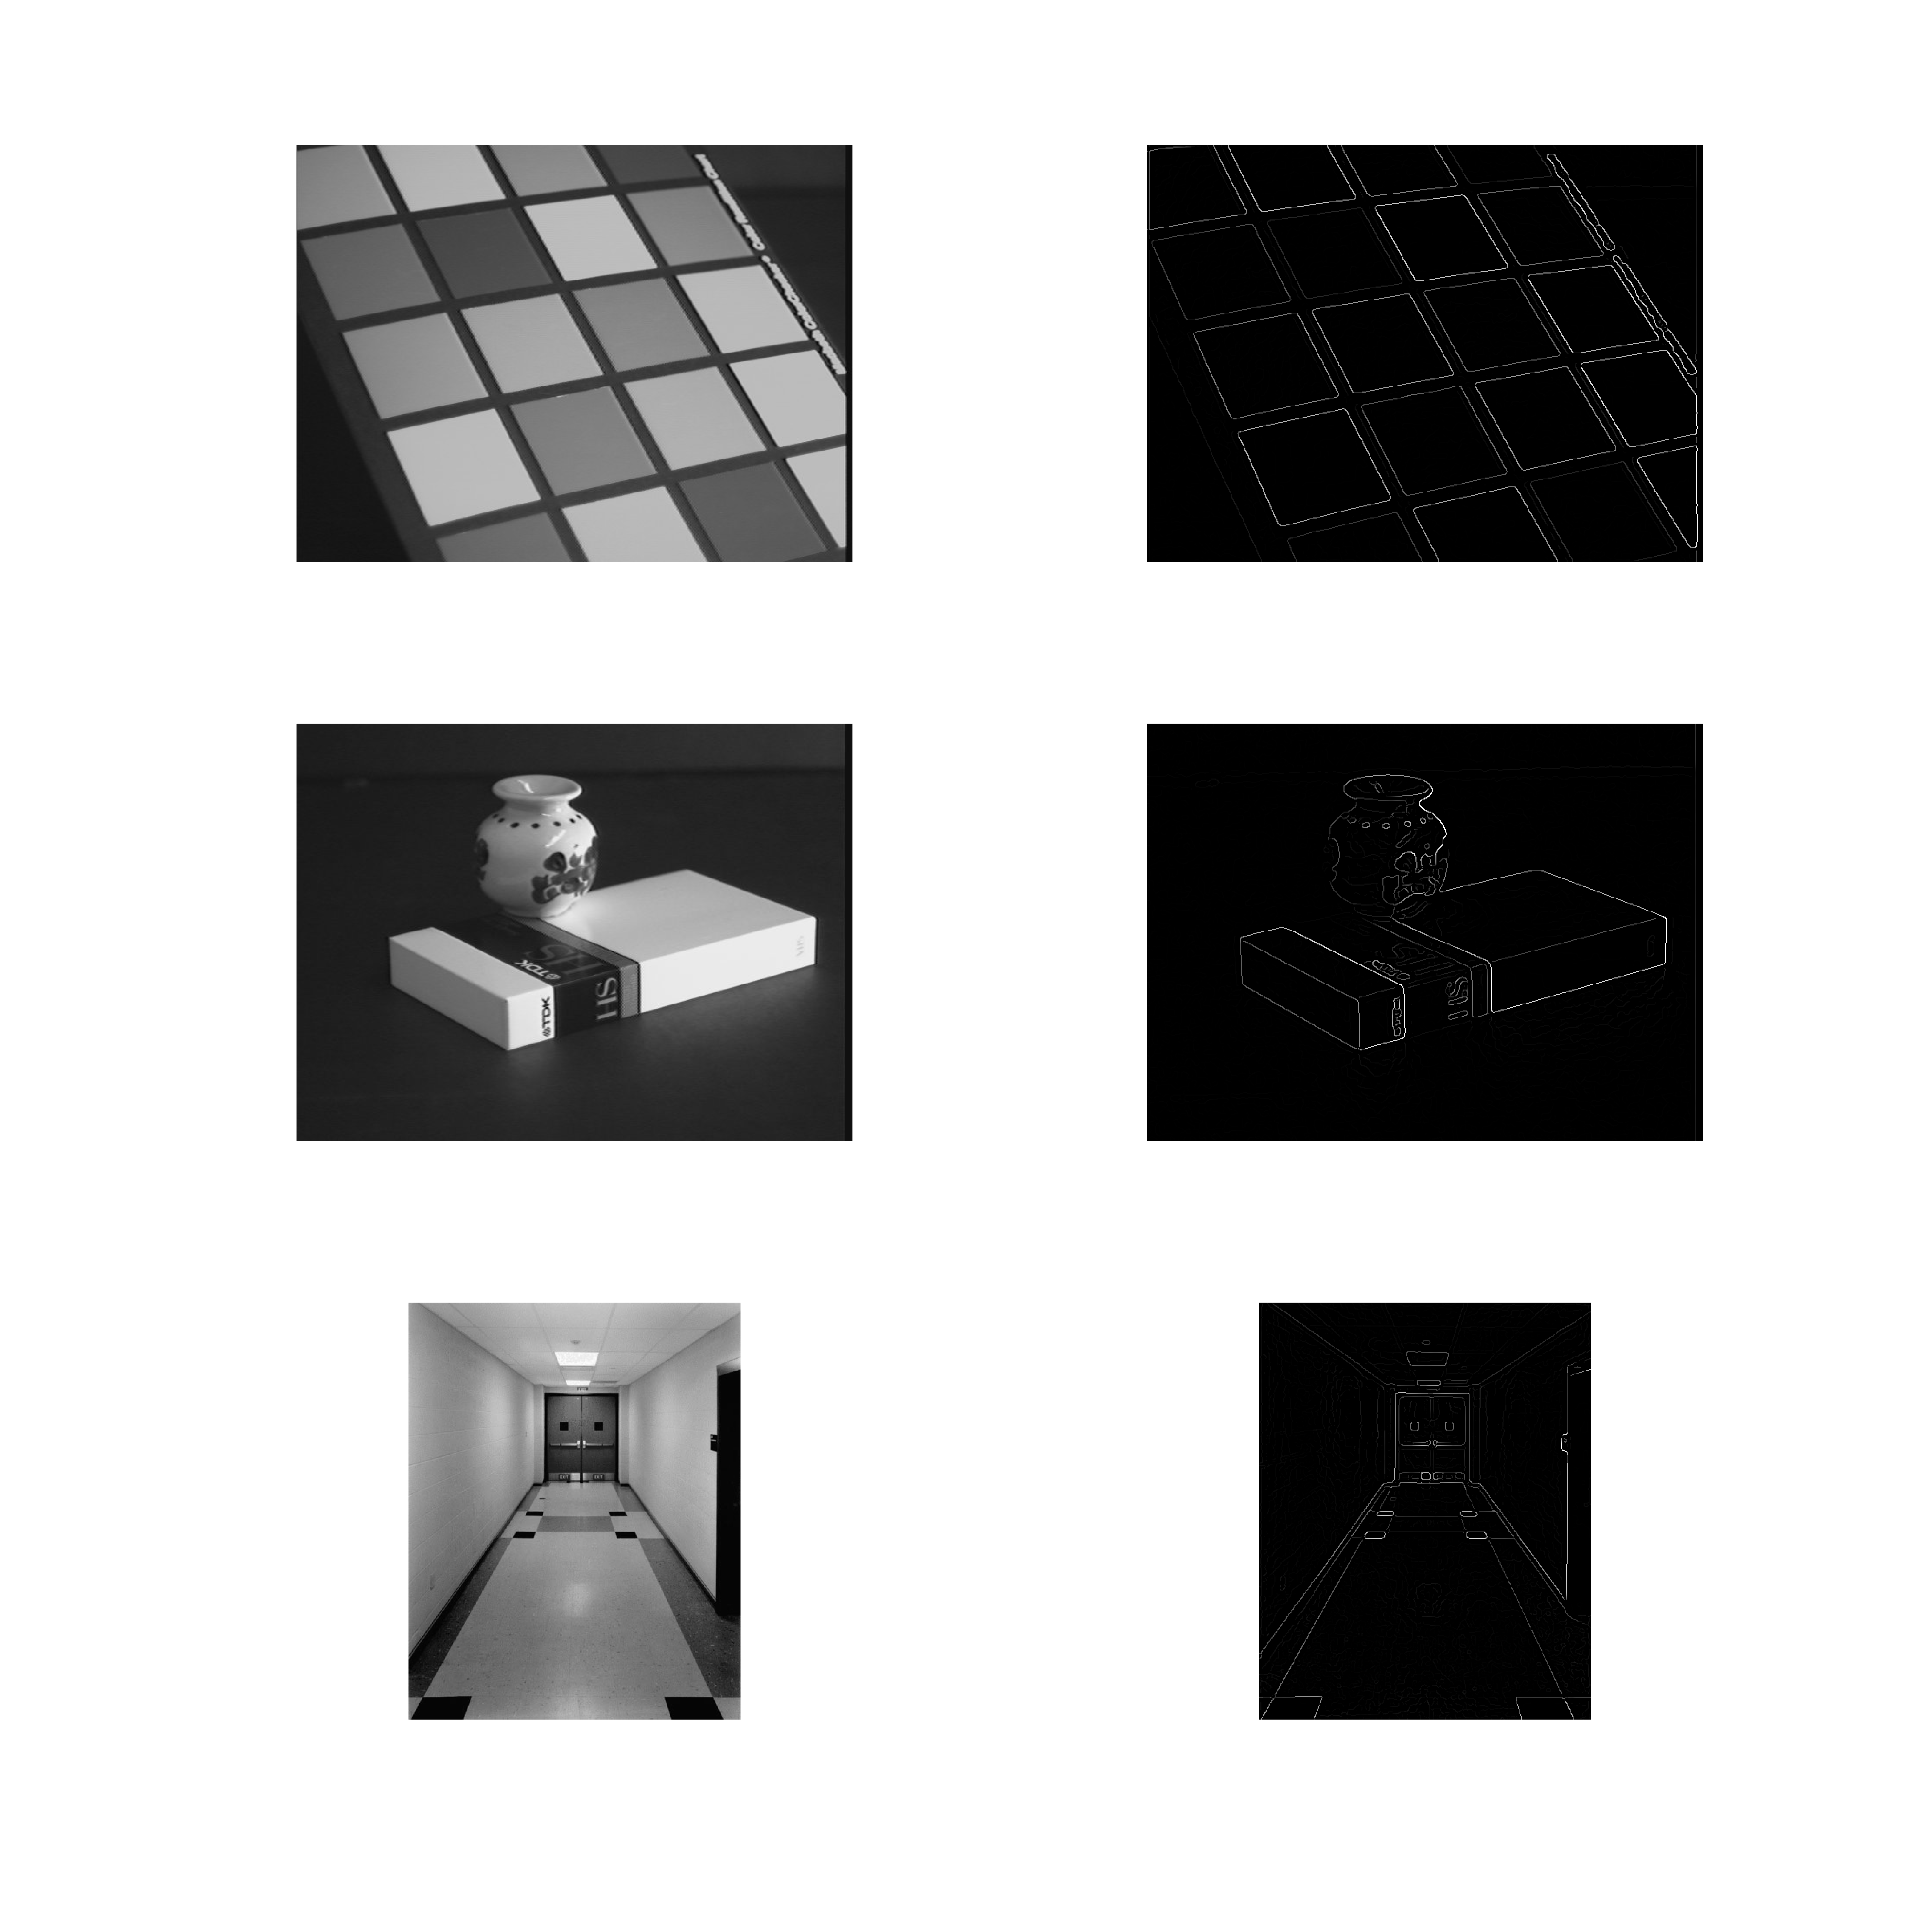
\includegraphics[width=\linewidth]{hw4_1_1}
    \caption{result of edge detection(right) given image(left)}
    \label{fig:1}
\end{figure}

Matlab code matlab/myEdgeFilter.m contains edge detection routine given greyscale image and standard deviation
of the gaussian kernel for smoothing the image before edge detection. Edge detection is composed of three stages;
first, the image is smoothed out so to prevent the noise to be detected as an edge component. Smoothing is done with
gaussian filter with the specified standard deviation. Next, Sobel filter is applied onto the smoothed image. In detail,
two first derivative filters, known as Sobel mask $S_x$, $S_y$ for horizontal/vertical changes, are applied onto the image. 

\[S_x = \begin{bmatrix}-1 & -2 & -1\\ 0 & 0 & 0\\ 1 & 2 & 1\end{bmatrix} , \quad
S_y = \begin{bmatrix}-1 & 0 & 1\\ -2 & 0 & 2\\ -1 & 0 & 1\end{bmatrix}\]
\[G_x = S_x \ast image , \quad G_y = S_y \ast image\]

The output are horizontal and vertical derivative approximations of the image, $G_x$ and $G_y$ respectively. 
Magnitude, angle gradient of the image $M$, $\alpha$ can be calculated with the equation below:

\[M = \sqrt{G_x^2 + G_y^2}\]
\[\alpha = tan^{-1}(\frac{G_y}{G_x})\]

Lastly, with non-maximum suppression (NMS), weak magnitude within a window is suppressed, producing thinner edge components.
NMS is processed as follows: for each pixel position $(x,y)$, its magnitude gradient $M(x,y)$ is compared with the magnitude of
its neighboring pixels in direction $\alpha(x,y)$ within a window. If $M(x,y)$ is smaller than any of the magnitudes along the
gradient line, $M(x,y)$ is suppressed. 

\begin{figure}[h]
    \centering
    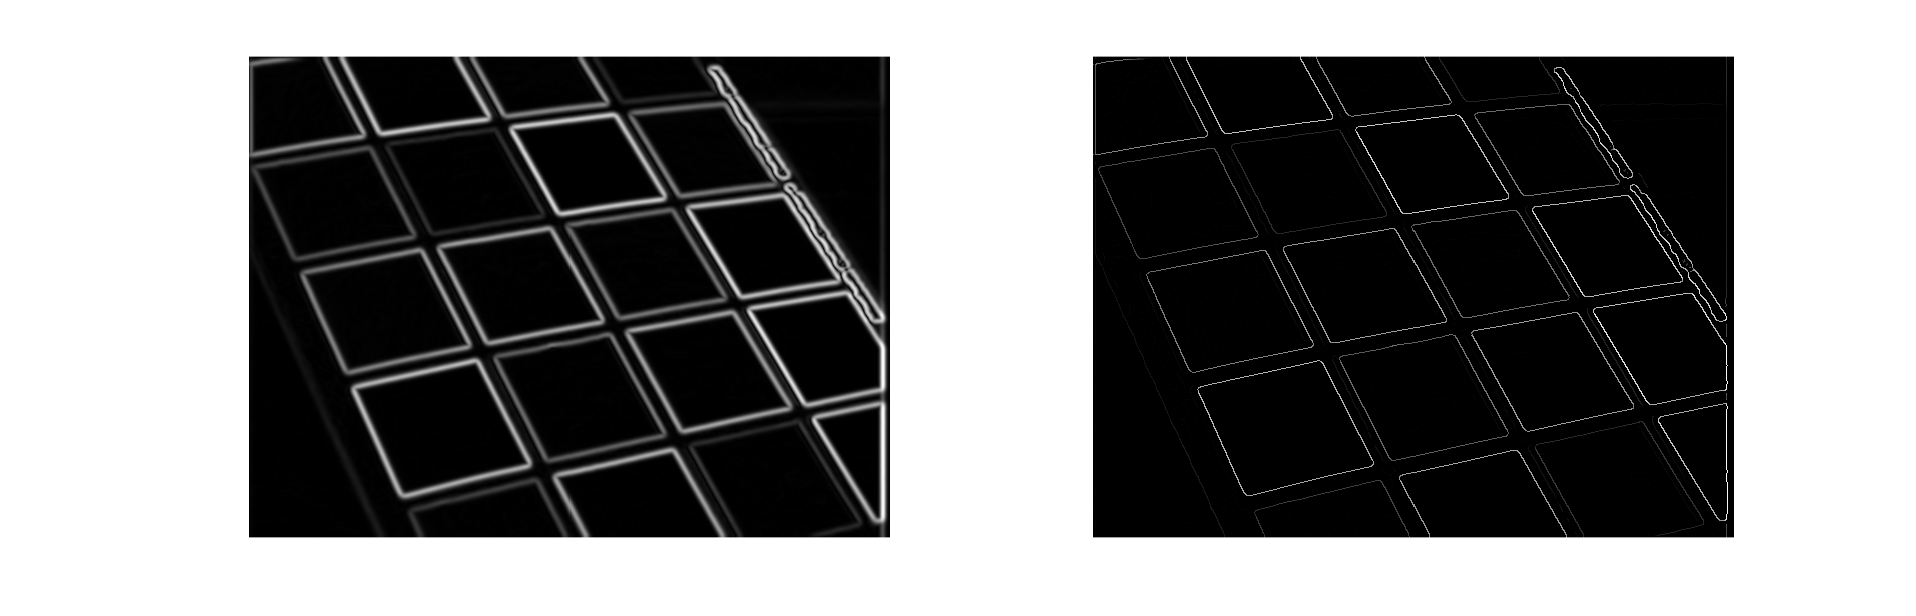
\includegraphics[width=\linewidth]{hw4_1_2}
    \caption{result of edge detection without NMS(left) and with NMS(right)}
    \label{fig:2}
\end{figure}

\figurename{\ref{fig:2}} contains the edge detection results of the given image with or without the NMS postprocessing.
It can be seen that compared to the original(left), postprocessed image(right) has much thinner edge components.

\section*{problem 2: the hough transform}

Matlab code matlab/myHoughTransform.m contains hough transform routine given edge image, threshold for ignoring small edge
filter response, resolution units for $\rho$ and $\theta$ for quantization. The implementation is based on the
Standard Hough Transform(SHT) that uses the parametric representation of a line as follows:
\[\rho = x * cos(\theta) + y*sin(\theta)\]

here $\rho$ is the distance between the line and the origin, $\theta$ is the angle of the projection from the origin to the line. 
\figurename{\ref{fig:3}} depicts the parametrization of a line in both planes. It can be seen that each point in xy-plane
can be represented as a sinusoiadal curve.  

\begin{figure}[h]
    \centering
    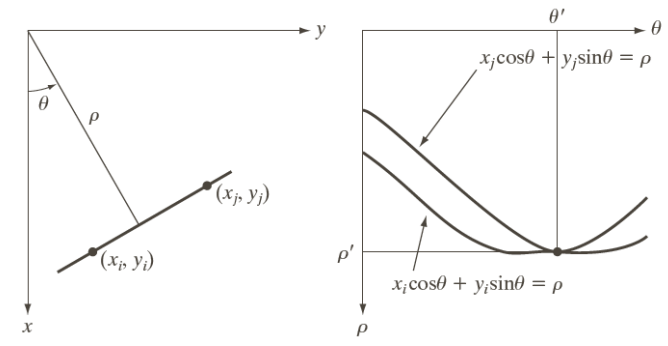
\includegraphics[width=\linewidth]{hw4_2_1}
    \caption{visualization of the parametric representation of a line in both xy-plane or $\rho\theta$-plane}
    \label{fig:3}
\end{figure}

Hough transform given thresholded edge filter response starts with building valid $\rho$ and $\theta$ values with
the resolution parameters; followed by the MATLAB implementation, in matlab/houghTransform.m, max/min value for 
the $rho$ is defined as:
\[D = \sqrt{(h-1)^2 + (w-1)^2}\]
\[min_{\rho} = -res_{\rho} * ceil(D / res_{\rho}) , \quad max_{\rho} = res_{\rho} * ceil(D / res_{\rho}) \]
where $h$, $w$ is the height, width of the given image and $res_{\rho}$ is the resolution unit of the $rho$.
Thus, the valid values for $\rho$ and $\theta$ are defined as below. Notice that $\theta$ is in degree unit in below equation.
\[scale_{\rho} = min_{\rho}:res_{\rho}:max_{\rho}\]
\[scale_{\theta} = -90:res_{\theta}:90-res_{\theta}\]

The hough transform matrix $H$ is $length(scale_{\theta}) \times length(scale_{\rho})$. Initially,
$H$ is set to zero. Then, for every pixel position $(x,y)$ in edge response, $\rho = x * cos(\theta) + y * sin(\theta)$ is calculated
for every $\theta$ in $scale_{\theta}$. $\rho$ is approximated as the value in $scale_{\rho}$, and $H(i_{\theta}, i_{\rho})$ is 
increased by 1 where $scale_{\theta}(i_{\theta}) = \theta$, $scale_{\rho}(i_{\rho}) = \rho$. 

\begin{figure}[h]
    \centering
    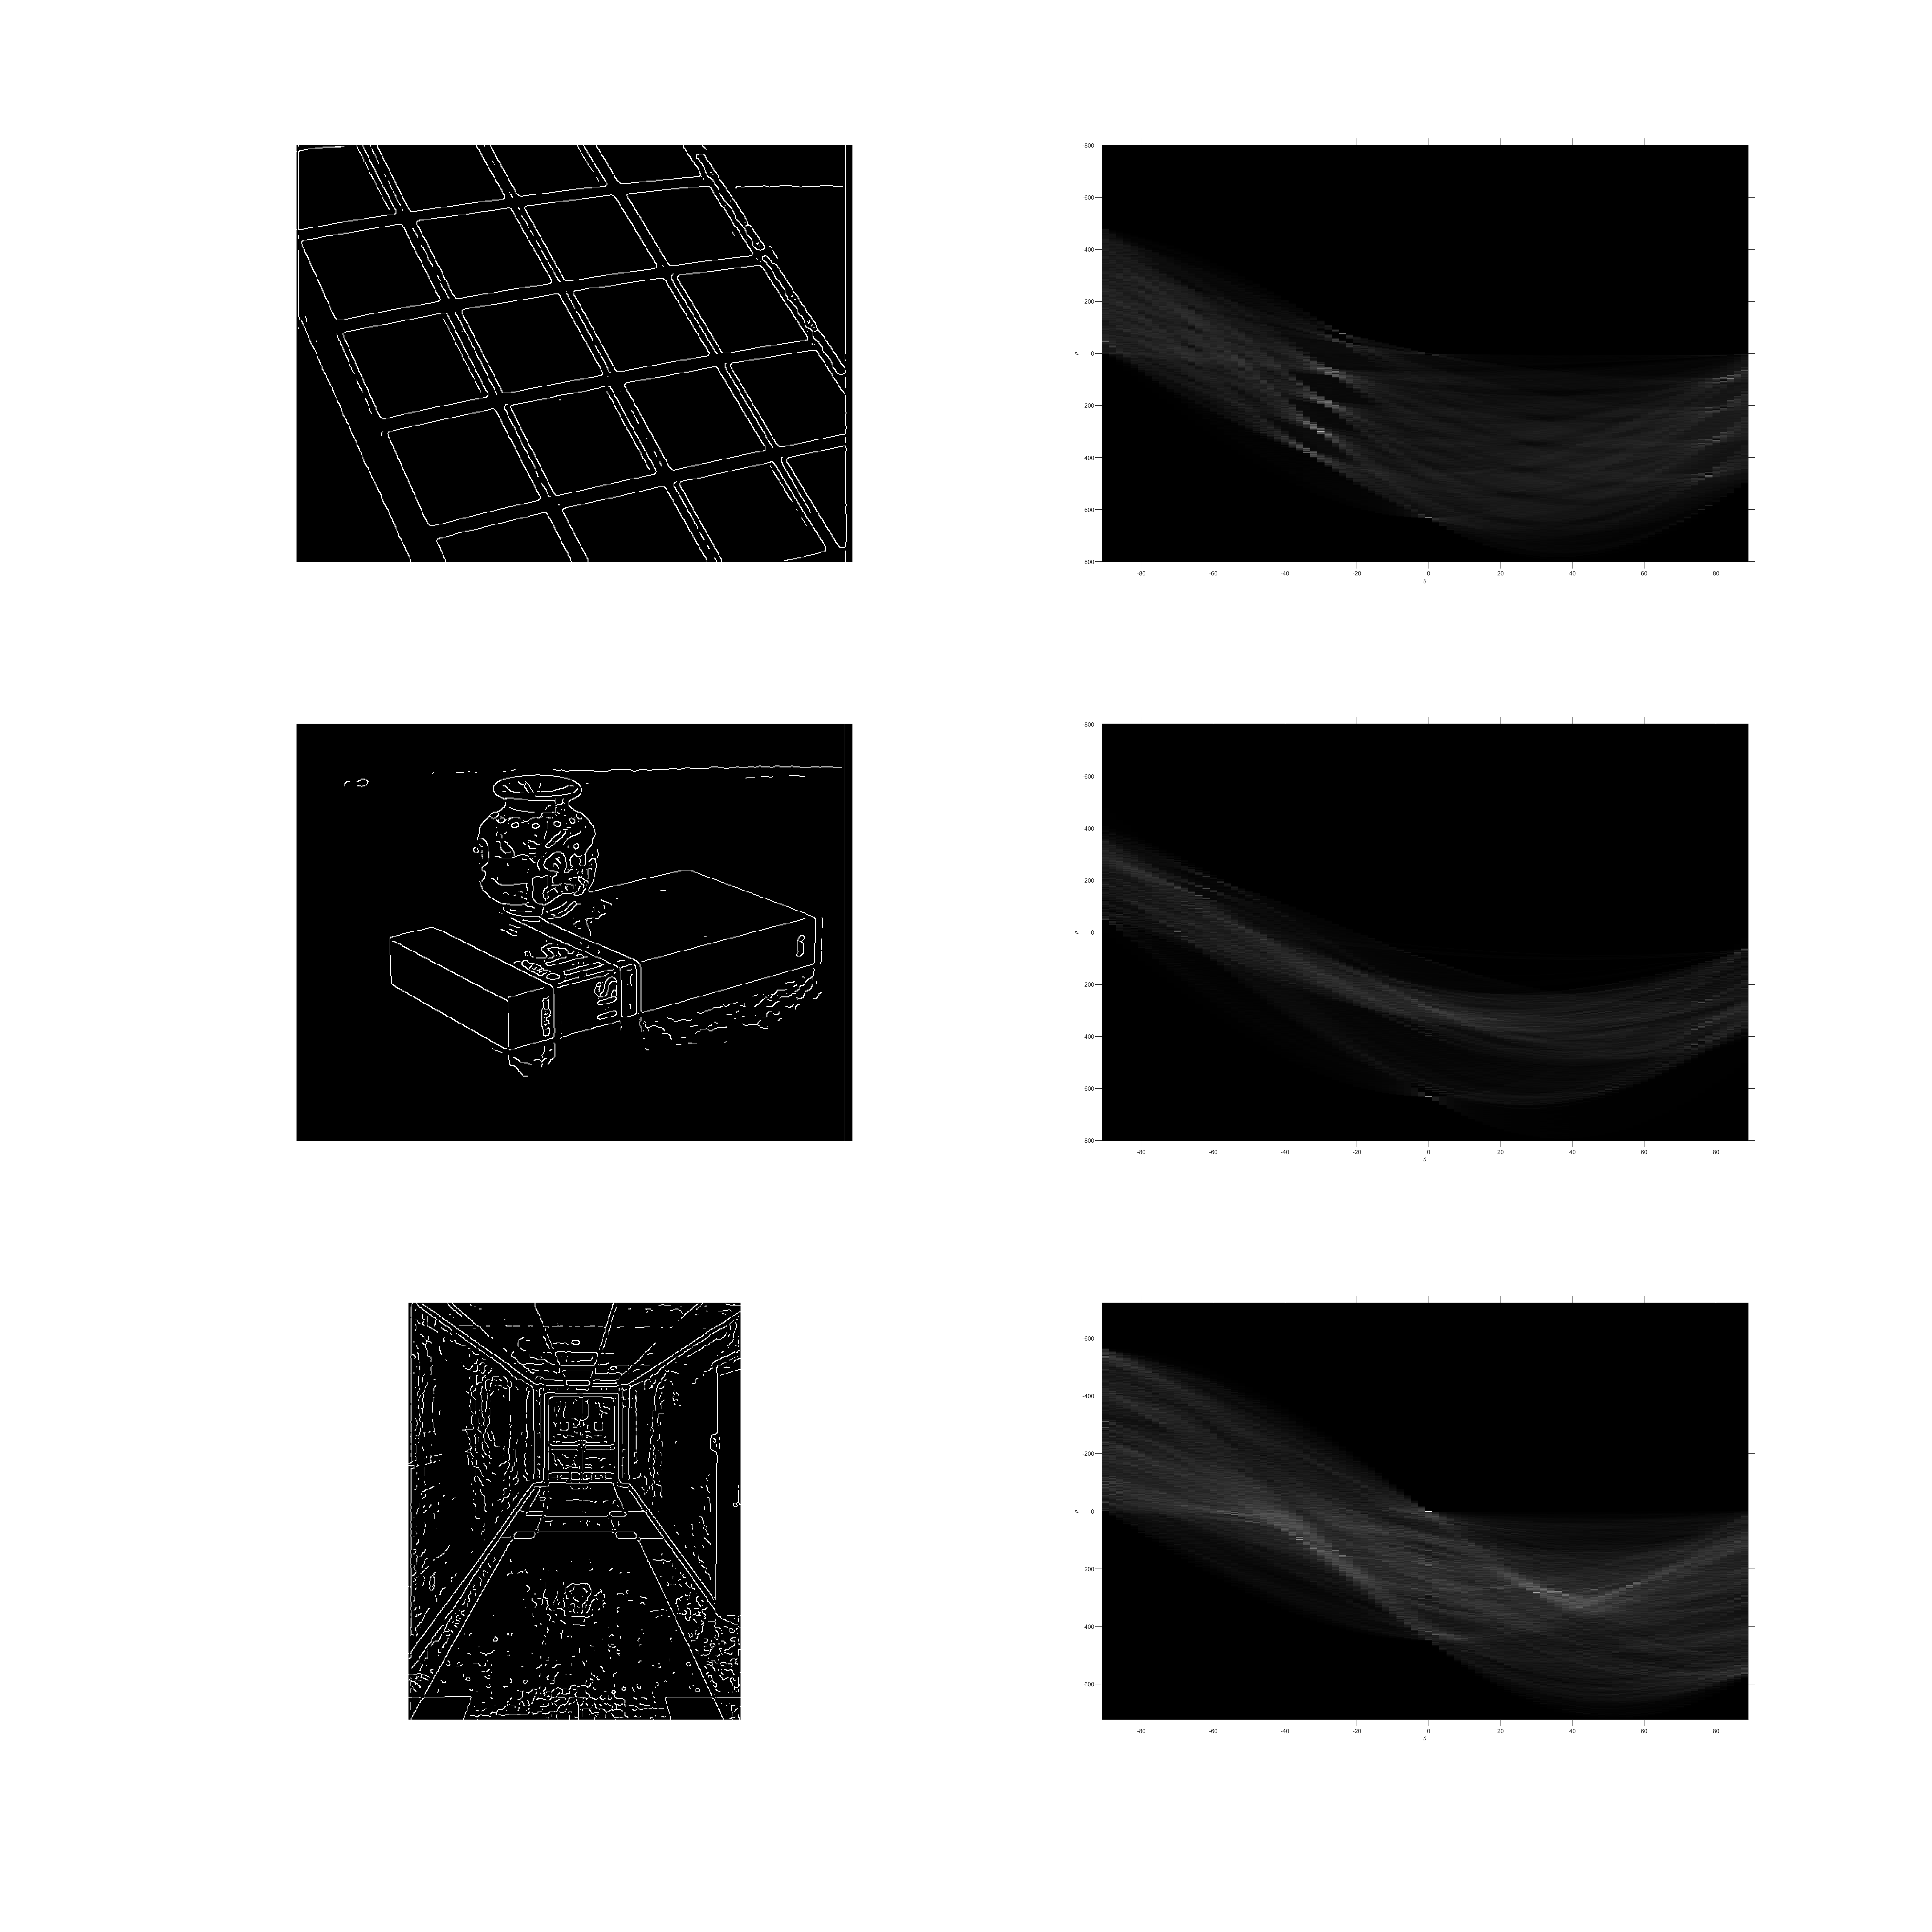
\includegraphics[width=\linewidth]{hw4_2_2}
    \caption{edge response and its hough transform of the given image. $res_{\rho} = 2$, $res_{\theta} = 2^{\circ}$}
    \label{fig:4}
\end{figure}

\figurename{\ref{fig:4}} depicts the hough transform given the edge response image. In $\theta$ range $-40 ~ -20$, high accumulation
is observed which can be one of the major lines. 

\section*{problem 3: finding lines}

Matlab code matlab/myHoughLines.m accepts the hough transform matrix $H$ and number of peaks to be extracted as input
arguments and returns the peak coordinates within $H$. The peak in $\rho\theta$ plane corresponds to a line in $xy$ plane.
Naive implementation of returning $\rho\theta$ indices of top $N$ values in $H$ where $N$ refers to the maximum number of
peaks to be found can generate thick lines, unwanted noises. Non-maximum suppression on $\rho\theta$ plane can help with
thinner lines while suppressing noisy lines. NMS can be done as follows: For each iteration, select the index 
$(i_{\rho} i_{\theta})$ from $H$ having the maximum value, and then set $H(i, j)$ as $0$ where $(i, j)$ is the indices 
within the window centered at $(i_{\rho}, i_{\theta})$.
Detailed algorithm can be found in Algorithm\ref{alg:2}.

\begin{algorithm}
    \caption{matlab/myHoughLines.m}
    \label{alg:2}
    \KwIn{$H$ of size $(M,N)$}
    \KwIn{$numLines$}
    $peaks = zeros(nLines, 2)$\;
    $threshold = 0.3 * max(H(:))$\;
    $radius = [4, 4]$\;
    \For{$i = 1:nLines$}{
        $[val, idx] = max(H(:))$\;
        \If{$val < thres$}{
            break\;
        }
        $[i_{\rho}, i_{\theta}] = ind2sub(size(H), idx)$\;
        push $[i_{\rho}, i_{\theta}]$ in $peaks$\;
        \For{$j = i_{\rho} - radius(1) : i_{\rho} + radius(1)$}{
            \For{$k = i_{\theta} - radius(2) : i_{\theta} + radius(2)$}{
                $H(j, k) = 0$\;
            }
        }
    }
    return $peaks(:, 1), peaks(:, 2)$\;
\end{algorithm}

\begin{figure}[h]
    \centering
    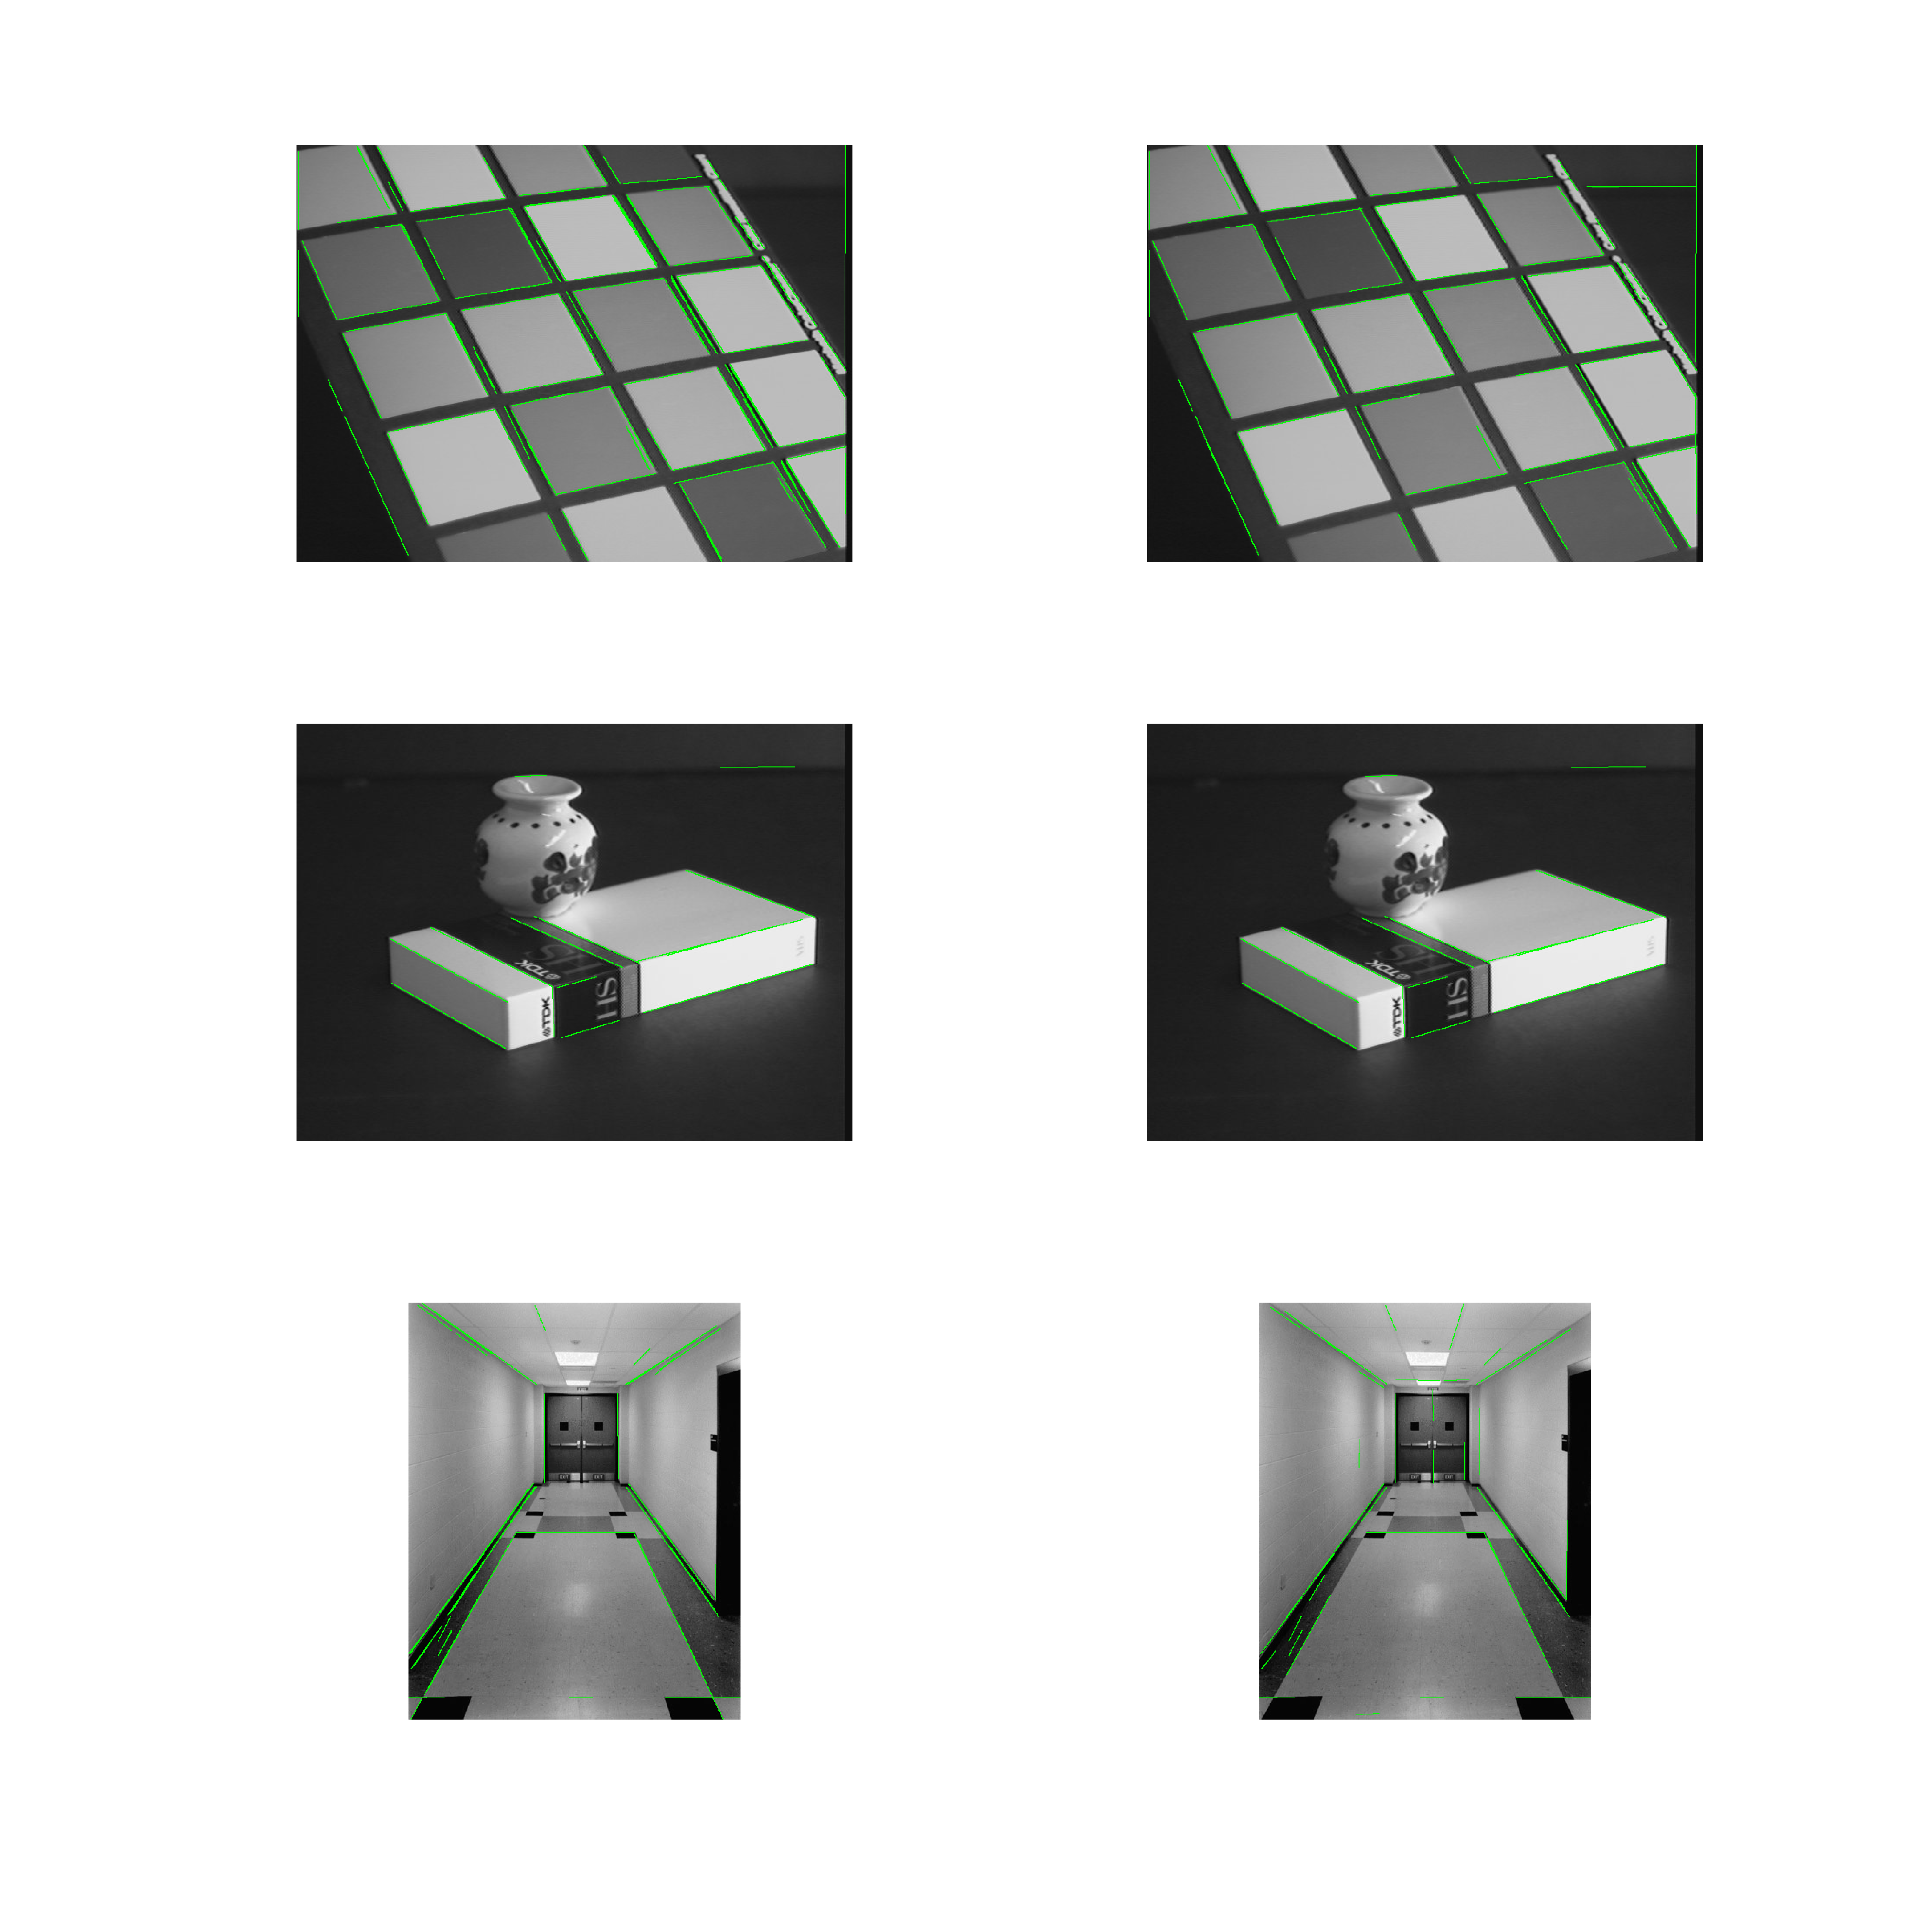
\includegraphics[width=\linewidth]{hw4_3_1}
    \caption{results of extracting peaks from $H$ given an image. 
    left: NMS postprocessing is applied on peak extraction; right: no postprocessing is done}
    \label{fig:5}
\end{figure}

\figurename{\ref{fig:5}} shows the effect of applying NMS on peak extraction. It can be seen from
the left of \figurename{\ref{fig:5}} that the lines become thinner with some noisy lines suppressed.

\section*{problem 4: hough circle transform}

The circle hough transform (CHT) is a specialization of hough transform, where the parametric equation
is based on circular equation. Given center point of a circle $(a, b)$ and $r$ as the radius, a circle
can be defined as:
\[(x-a)^2 + (y-b)^2 = r^2\]

By the equation, $xy$-plane can be mapped to 3-dimensional $(a, b, r)$ space. As in \figurename{\ref{fig:6}},
a circle in $xy$-plane is mapped to the surface of an inverted cone having apex $(x, y, 0)$.

\begin{figure}[h]
    \centering
    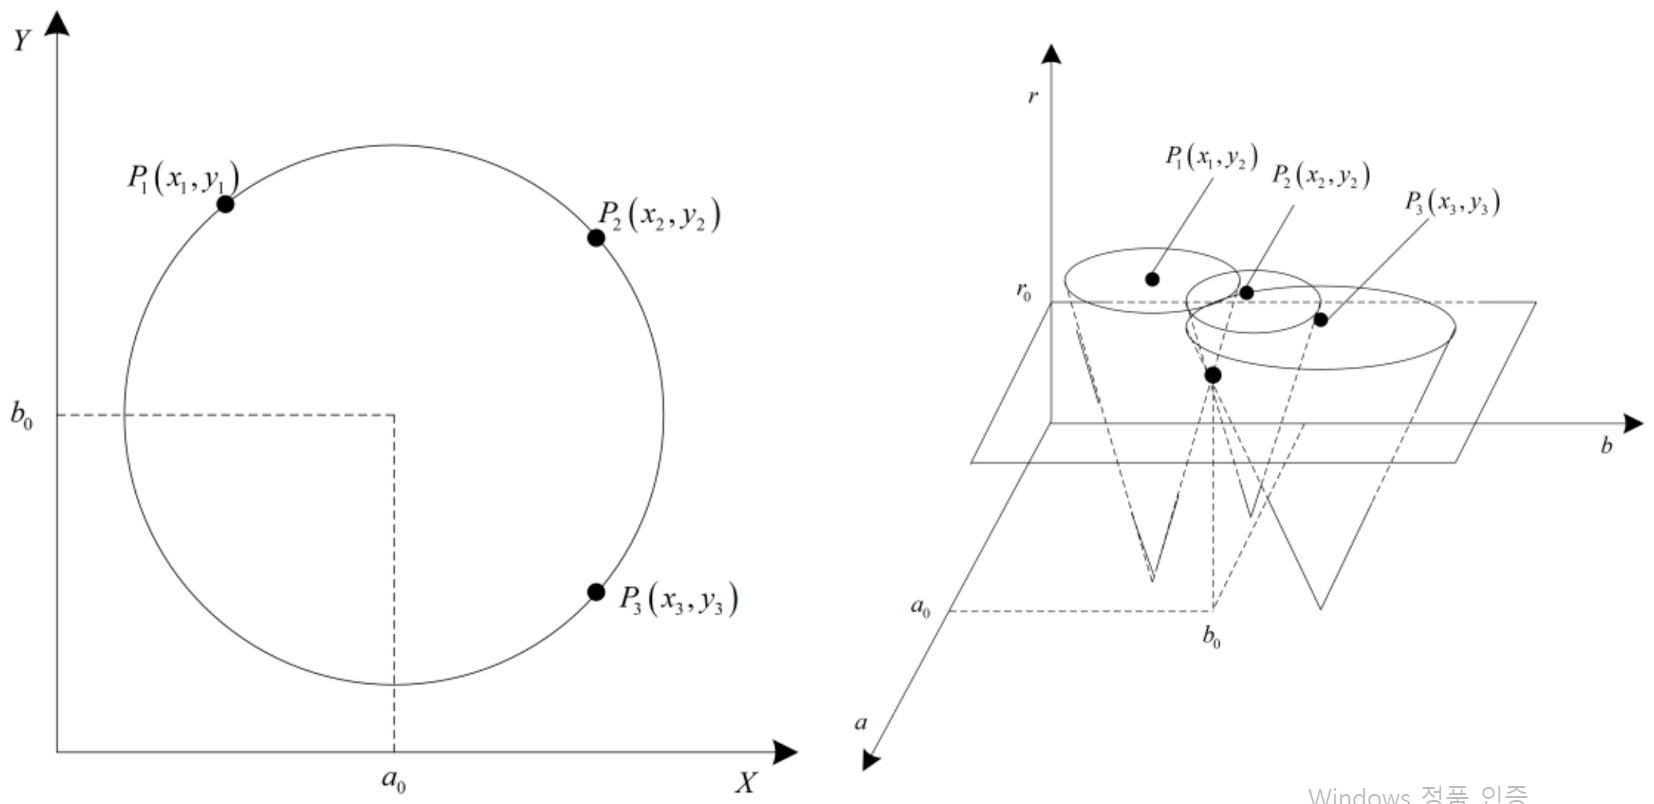
\includegraphics[width=\linewidth]{hw4_4_1}
    \caption{circular equation in $xy$ plane(left) and parametric space(right)}
    \label{fig:6}
\end{figure}

As in SHT, finding maximum intersections between the surfaces of the cones in $(a, b, r)$ space can be inverted
to the strong circular component in $xy$-plane. However, since the parametric space is 3-dimensional, the process of
finding maximum intersections can be divided into two stages; first, with predefined radius, find the optimal center
of the circles from $ab$-plane, then find the optimal radius given the circle centers from $r$-line. 

\begin{figure}[h]
    \centering
    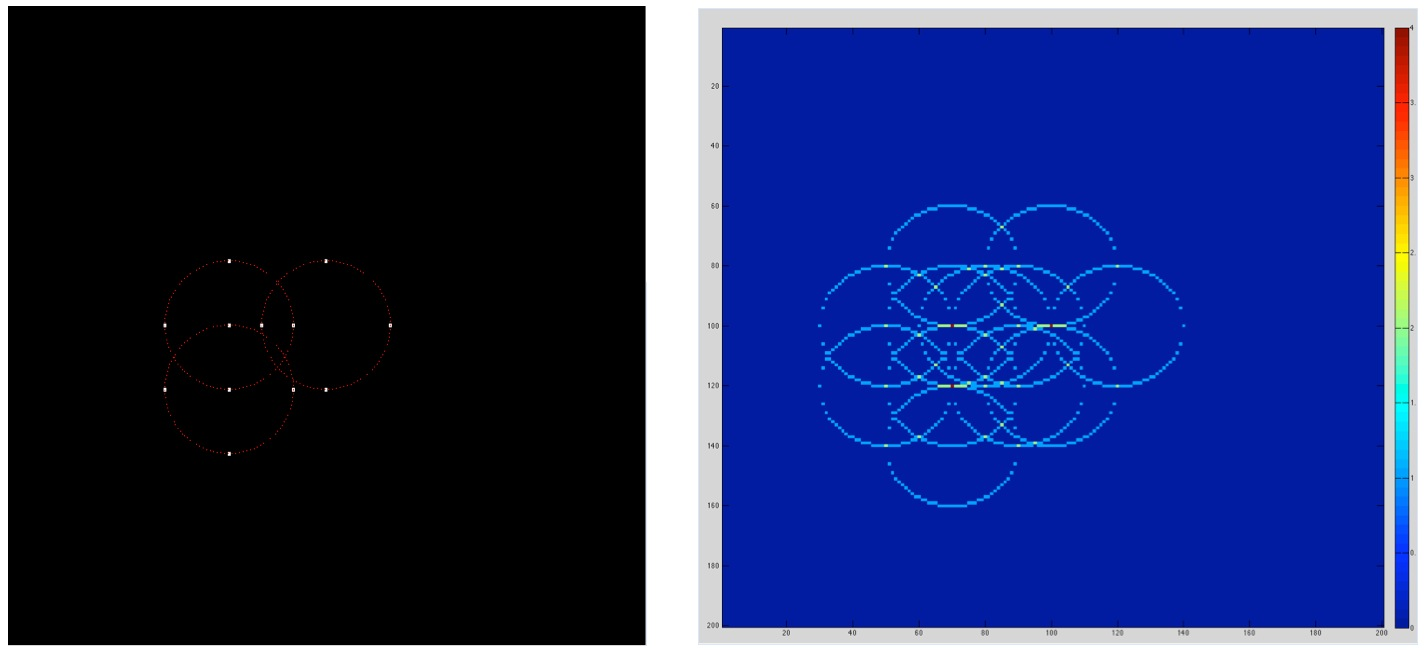
\includegraphics[width=\linewidth]{hw4_4_2}
    \caption{arbitrary points in $xy$-plane(left) and its parametric representation in $ab$-plane(right)
    assumed that the radius $r$ is known in advance}
    \label{fig:7}
\end{figure}

\figurename{\ref{fig:7}} shows the example of mapping between $xy$-plane and $ab$-plane with known radius $r$.
As in SHT, maximum intersection from the parametric representations, depicted as red dots in $ab$-plane,
can be inverted back to $xy$-plane defining the center of major circles from the scattered data.

In case the radius is unknown, iterating over 3-dimensional parametric space to find the maximum intersections
is also possible, while 3-dimensional accumulation is costly in terms of both memory and latency. 

\begin{figure}[h]
    \centering
    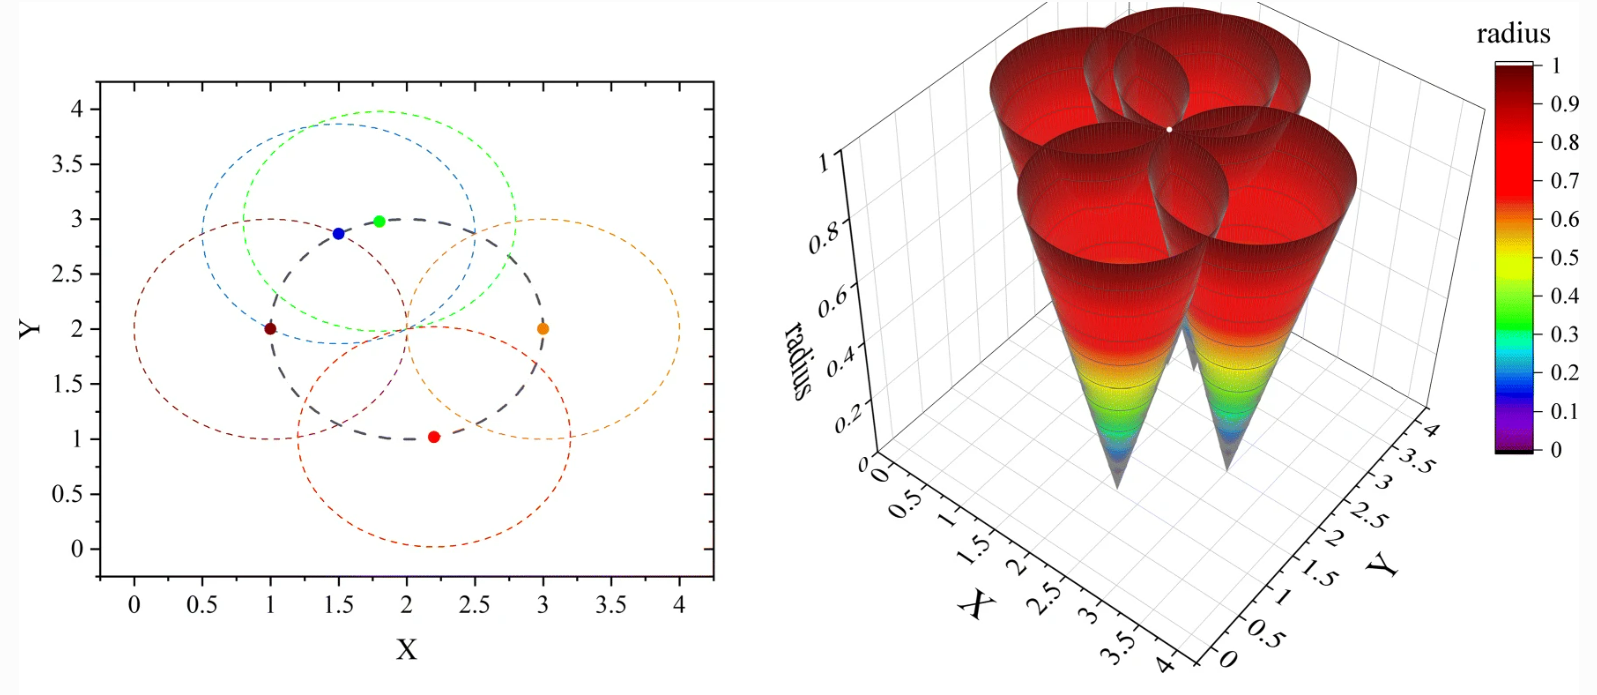
\includegraphics[width=\linewidth]{hw4_4_3}
    \caption{arbitrary points in $xy$-plane(left) and its parametric representation in $(a, b, r)$ space(right)}
    \label{fig:8}
\end{figure}

\figurename{\ref{fig:8}} shows the example of mapping between $xy$-plane and $(a, b, r)$ space. While dot in the
parametric space defines both the radius $r$ and the center of the circle $(a, b)$ in $xy$-plane.

\begin{figure}[h]
    \centering
    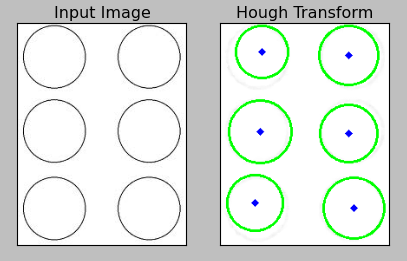
\includegraphics[width=\linewidth]{hw4_4_4}
    \caption{original image containing several circles and its CHT result}
    \label{fig:9}
\end{figure}

The example of applying CHT onto the image of multiple circles is shown in \figurename{\ref{fig:9}}. It can be 
seen that both circle center and its radius is approximated precisely.

\end{document}
